
%Talk given virtually to Mac Hyman and friends, November 15, 2021
\documentclass[10pt,compress,xcolor={usenames,dvipsnames},aspectratio=169]{beamer}
%\documentclass[xcolor={usenames,dvipsnames},aspectratio=169]{beamer} %slides and 
%notes
\usepackage{amsmath,
	amssymb,
	datetime,
	mathtools,
	bbm,
	%mathabx,
	array,
	booktabs,
	xspace,
	multirow,
	calc,
	colortbl,
	siunitx,
 	graphicx}
\usepackage[usenames]{xcolor}
\usepackage[giveninits=false,backend=biber,style=nature, maxcitenames =10, mincitenames=9]{biblatex}
\addbibresource{FJHown23.bib}
\addbibresource{FJH23.bib}
\usepackage{newpxtext}
\usepackage[euler-digits,euler-hat-accent]{eulervm}
\usepackage{media9}
\usepackage[autolinebreaks]{mcode}
\usepackage[tikz]{mdframed}


\usetheme{FJHSlimNoFoot169}
\setlength{\parskip}{2ex}
\setlength{\arraycolsep}{0.5ex}


\DeclareMathOperator{\SOL}{SOL}
\DeclareMathOperator{\APP}{APP}
\DeclareMathOperator{\ERR}{ERR}
\DeclareMathOperator{\AVG}{AVG}
\DeclareMathOperator{\INT}{INT}
\DeclareMathOperator{\LIN}{LINEAR}
\DeclareMathOperator{\BAD}{BAD}
%\DeclareMathOperator{\opt}{opt}
\newcommand{\dataN}{\bigl(\hf(\vk_i)\bigr)_{i=1}^n}
\newcommand{\dataNj}{\bigl(\hf(\vk_i)\bigr)_{i=1}^{n_j}}
\newcommand{\dataNjd}{\bigl(\hf(\vk_i)\bigr)_{i=1}^{n_{j^\dagger}}}
\newcommand{\ERRN}{\ERR\bigl(\dataN,n\bigr)}
\newcommand{\otod}{\ensuremath{1\mkern-4mu : \mkern-2mu d}}


%\DeclareMathOperator{\app}{app}

\providecommand{\HickernellFJ}{H.\xspace}


\renewcommand{\OffTitleLength}{-7ex}
\setlength{\FJHThankYouMessageOffset}{-8ex}
\title{Reproducing Kernels}
\author[]{Fred J. Hickernell}
\institute{Department of Applied Mathematics \qquad
	Center for Interdisciplinary Scientific Computation \\
	Office of Research \\  
	Illinois Institute of Technology \qquad
	\href{mailto:hickernell@iit.edu}{\url{hickernell@iit.edu}} \qquad
	\href{http://mypages.iit.edu/~hickernell}{\url{mypages.iit.edu/~hickernell}}}

\thanksnote{Thanks to Mac Hyman for the invitation \\
Thanks to many students and collaborators \\
Slides available at \href{https://speakerdeck.com/fjhickernell/reproducing-kernel-tutorial}{\nolinkurl{speakerdeck.com/fjhickernell/reproducing-kernel-tutorial}} \\
Please interrupt and ask questions}
	
%\event{Happy Fred}
\date[]{November 15, 2021}

\input FJHDef.tex



\begin{document}
	\everymath{\displaystyle}

\frame{\titlepage}

%%%%%%%%%%%%%%%%%%%%%%%%%%%%%%%%%%%%%%%%%%
%%%%%%%%%%%%%%%%%%%%%%%%%%%%%%%%%%%%%%%%%%
\section{Background}
%%%%%%%%%%%%%%%%%%%%%%%%%%%%%%%%%%%%%%%%%%
%%%%%%%%%%%%%%%%%%%%%%%%%%%%%%%%%%%%%%%%%%

\begin{frame}{What Can We Do with Reproducing Kernel Hilbert Spaces?}

\vspace{-5ex}
	\begin{itemize}
		\item Use the \alert{Reisz Representation Theorem} to derive \alert{error bounds} for algorithms for linear problems, such as integration, function approximation, solving linear differential equations%
				\uncover<2->{, \alert{BUT}
			\begin{itemize}
				\item You must be able to solve the problem for your reproducing kernel
				\item You must pick a kernel that matches your input function
				\item You may need to tune the kernel parameters
		\end{itemize}}
		
		\item Derive \alert{optimal} algorithms%
		\uncover<2->{, \alert{BUT} it takes $\Order(n^3)$ operations to compute the weights}
		\item Determine \alert{how fast} the error bounds decay to zero as the computational effort increases, and even whether convergence depends significantly on the \alert{number of variables}
		\item Include \alert{trends}\uncover{, \alert{BUT} I  have not prepared that for today.}
		\item Derive a parallel analysis using \alert{Gaussian processes} where the reproducing kernel is interpreted as a \alert{covariance kernel}
				\uncover<2->{, \alert{BUT} I have not prepared that for today}
	\end{itemize}	

\end{frame}



%%%%%%%%%%%%%%%%%%%%%%%%%%%%%%%%%%%%%%%%%%
%%%%%%%%%%%%%%%%%%%%%%%%%%%%%%%%%%%%%%%%%%
\section{Rep Ker \& Riesz Rep Thm}
%%%%%%%%%%%%%%%%%%%%%%%%%%%%%%%%%%%%%%%%%%
%%%%%%%%%%%%%%%%%%%%%%%%%%%%%%%%%%%%%%%%%%

\begin{frame}[label = RKRd]{Reproducing Kernels for Functions on $\{1, \ldots, d\}$, aka Vectors}

\vspace{-3ex}
Let $\cf$ \uncover<1-3>{$:=$ all functions on $\{1, \ldots, d\} \text{ ``$=$'' } \reals^d$}\uncover<4>{ be a vector space of functions}\\
\uncover<1-3>{Pick a symmetric, positive definite (positive eigenvalues) matrix $\mW \in \reals^{d \times d}$ to} define an inner product \vspace{-0.3ex}
\[
\only<1-3>{\ip{f}{h} : = \vf^T \mW \vh, \quad \forall f, h \in \cf, \qquad \text{where } \vf = \bigl(f(t) \bigr)_{t=1}^d} \only<4>{\alert{\mW \text{ is gone}}} \vspace{-0.7ex}
\]
\uncover<2-4>{\alert{Reproducing kernel}, $K$, \uncover<1-3>{is defined by 
$\bigl ( K(t,x) \bigr)_{t,x=1}^d = \mK := \mW^{-1}$, and }has the properties
\vspace{-0.5ex}
\begin{gather*}
    \alert{\text{Symmetry }} K(t,x) = K(x,t) \uncover<1-3>{\text{ because $\mW$ is symmetric and thus so is $\mK$}} \\
    \alert{\text{Positive Definiteness }} \bigl(  K(x_i,x_j)\bigr)_{i,j = 1}^n \text{ is positive definite for any distinct } x_1, \ldots, x_n \in \{1, \ldots, d\}\\
     \alert{\text{Belonging }} K(\cdot,x)\uncover<1-3>{ = \text{$x^{\text{th}}$ column of $\mK$} =: \vK_x} \in \cf\\
    \alert{\text{Reproduction }} \ip{K(\cdot,x)}{f} \uncover<1-3>{= \vK_x^T \mW \vf = \ve_x \vf} = f(x) \uncover<1-3>{\quad \text{since } \mK := \mW^{-1};  \qquad 
 \ve_x := (0, \ldots, 0, \underbrace{1}_{x^{\text{th}} \text{ position}}, 0, \ldots )^T}
\end{gather*}
\uncover<3->{\alert{Riesz Representation Theorem} says that \uncover<1-3>{for any linear function, $\LIN$, there is a \alert{representer} $g$ such that} $\LIN(f) = \ip{g}{f}\uncover<1-3>{ = \vg^T \mW \vf}$\uncover<1-3>{.  Note}
\[
\begin{pmatrix} g(1) \\ \vdots \\ g(d)\end{pmatrix} 
\uncover<1-3>{= \vg = \mK \mW \vg 
= \begin{pmatrix} \mK_1^T \mW \vg \\ \vdots \\ \mK_d^T \mW \vg\end{pmatrix}
= \begin{pmatrix} \ip{K(\cdot,1)}{g} \\ \vdots \\ \ip{K(\cdot,d)}{g} \end{pmatrix}}
= \begin{pmatrix} \LIN(K(\cdot,1)) \\ \vdots \\  \LIN(K(\cdot,d)) \end{pmatrix}
\]
}
}


\end{frame}


\begin{frame}{Reproducing Kernels for Functions on General Domains  \cite{Aro50}}

\vspace{-4ex}
	Suppose that  $(\cf,\ip{\cdot}{\cdot})$  is a Hilbert space of functions on $\Omega$ for which \alert{function evaluation is bounded}.  Then there exists a \alert{unique reproducing kernel}  $K: \Omega \times \Omega \to \reals$ for which 
	\vspace{-1ex}
	\begin{gather*}
		\underbrace{K(\vt,\vx) = K(\vx,\vt)}_{\alert{\text{symmetry}}},  \quad \underbrace{K(\cdot,\vx) \in \cf}_{\alert{\text{belonging}}}, \quad  \underbrace{f(\vx) = \ip{K(\cdot,\vx)}{f}}_{\alert{\text{reproduction}}}  \qquad \forall \vt, \vx \in \Omega, \; f \in \cf \\
		K(\mX,\mX) = \bigl(K(\vx_i,\vx_j)\bigr)_{i,j = 1}^n \text{ is \alert{positive definite} for any $n \times d$ $\mX$ with distinct rows lying in $\Omega$}
	\end{gather*}
	
	\vspace{-3ex}
	$\cf$ is the completion of $\{c_1 K(\cdot,\vx_1) + \cdots + c_nK(\cdot, \vx_n) : n \in \naturals, \vc \in \reals^n\}$; any $K$ satisfying the above implies $\cf$
	
\uncover<2->{\alert{Riesz Representation Theorem} says that for any bounded $\LIN : \cf \to \reals$ there exists a \alert{representer} $g \in \cf$ such that $\LIN(f)  =  \ip{g}{f} $ for all $f \in \cf$.  \alert{What is $g$?}
\uncover<3->{
\begin{gather*}
	g(\vx) \underbrace{=}_{\text{reproduction}} \ip{K(\cdot,\vx)}{g} \underbrace{=}_{\text{symmetry}}  \ip{g}{K(\cdot,\vx)} \underbrace{=}_{\text{representer}} \LIN\bigl(K(\cdot,\vx)\bigr) \qquad \forall \vx \in \Omega\\
		\uncover<4->{\norm{g}^2 = \ip{g}{g} \underbrace{=}_{\text{representer}} \LIN(g) = \LIN^{\cdot\cdot} \bigl( \LIN^\cdot\bigl(K(\cdot,\cdot \cdot)\bigr)   \bigr)
		}
\end{gather*}

\vspace{-3ex}
\uncover<4->{\alert{Do not} need the definition of $\ip{\cdot}{\cdot}$ to compute $g$ and $\norm{g}$}
}
}

\end{frame}

%%%%%%%%%%%%%%%%%%%%%%%%%%%%%%%%%%%%%%%%%%
%%%%%%%%%%%%%%%%%%%%%%%%%%%%%%%%%%%%%%%%%%
\section{Kernel Ex}
%%%%%%%%%%%%%%%%%%%%%%%%%%%%%%%%%%%%%%%%%%
%%%%%%%%%%%%%%%%%%%%%%%%%%%%%%%%%%%%%%%%%%
\begin{frame}{Squared Exponential Kernel on $\reals$}
	
	\vspace{-8ex}
\begin{tabular}{m{0.5\textwidth}m{0.5\textwidth}}
	The squared exponential (aka Gaussian) kernel for univariate functions takes the form 
	\[
	K(t,x) = A \exp\bigl(-\gamma^2\abs{t-x}^2 \bigr) , \qquad t, x \in \reals
	\]
corresponds to the Hilbert space of functions with norm \cite[(6.18)]{RasWil06a}
\begin{equation*}
\norm{f}^2 = A\sqrt{\pi} \sum_{m=0}^\infty\frac{\int_{\reals} \abs{f^{(m)}(x)}^2 \, \dif x}{m! 4^m \gamma^{2m+1}}
\end{equation*}
which means that functions  have all deriviatives square integrable.
&
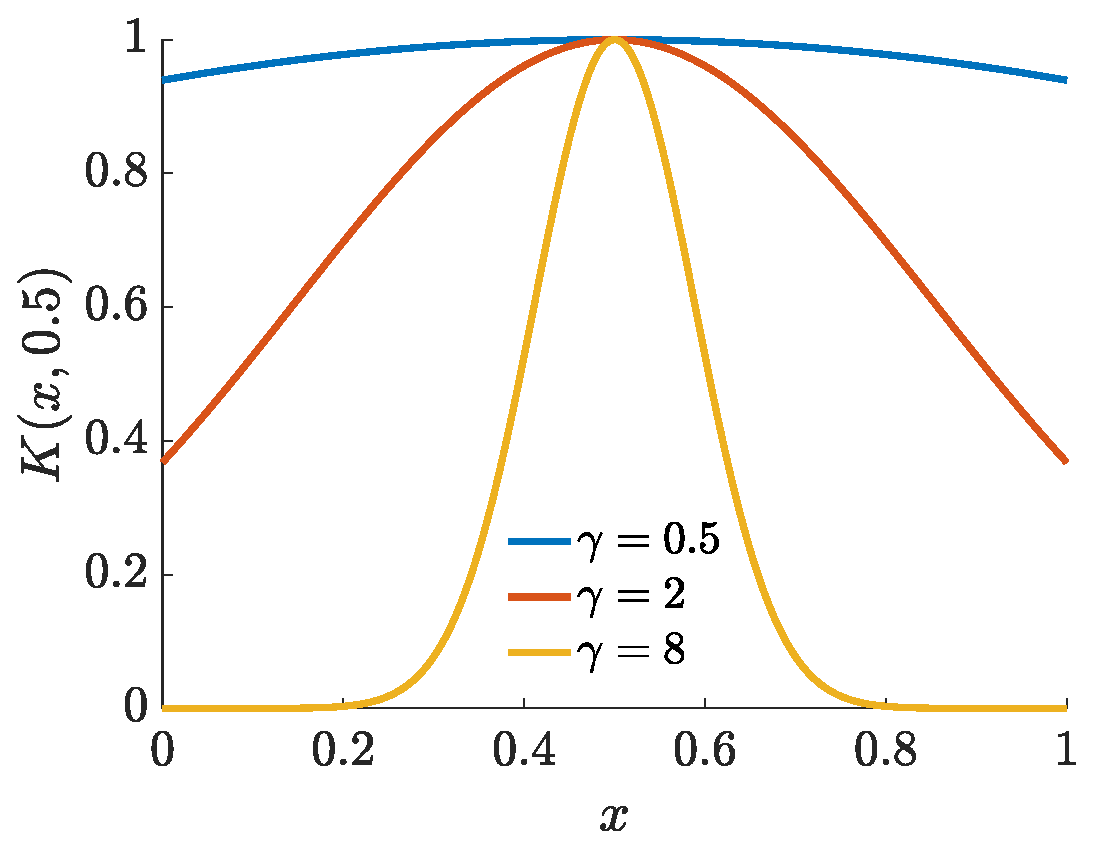
\includegraphics[width=0.45\textwidth]{RK-sqexpker.eps}
\end{tabular}
\end{frame}

\begin{frame}{Squared Exponential Kernel on $\reals^d$}
	
\vspace{-4ex}
\begin{tabular}{m{0.6\textwidth}m{0.4\textwidth}}
	The squared exponential kernel for $d$-variate functions takes the form 
	
	\vspace{-4ex}
	\begin{multline*}
	K(\vt,\vx) = A \exp\bigl(-\gamma_1^2\abs{t_1-x_1}^2 - \cdots - \gamma_d^2\abs{t_d-x_d}^2 \bigr) , \\
	 \vt, \vx \in \reals^d
	\end{multline*}

	\vspace{-1ex}
	corresponds to the Hilbert space of functions with norm

	\vspace{-4ex}
	\begin{gather*}
		\norm[2]{D^{\vm} f}^2 := \int_{\reals^d} \abs{\frac{\partial^{\norm[1]{\vm}}f(\vx)}{\partial x_1^{m_1} \cdots \partial x_d^{m_d}}}^2 \, \dif \vx \\
		\norm{f}^2 =  A\sqrt{\pi}  \sum_{\vm \in \natzero^d} \frac{\norm[2]{D^{\vm} f}^2}{\norm[1]{\vm}! \, 4^{\norm[1]{\vm}} \prod_{k=1}^d \gamma_k^{2m_j}}
	\end{gather*}
	which means that functions have all deriviatives square integrable.  This kernel is \alert{stationary}.  It is \alert{isotropic} if  $\gamma_1 = \cdots = \gamma_d$.
	&
	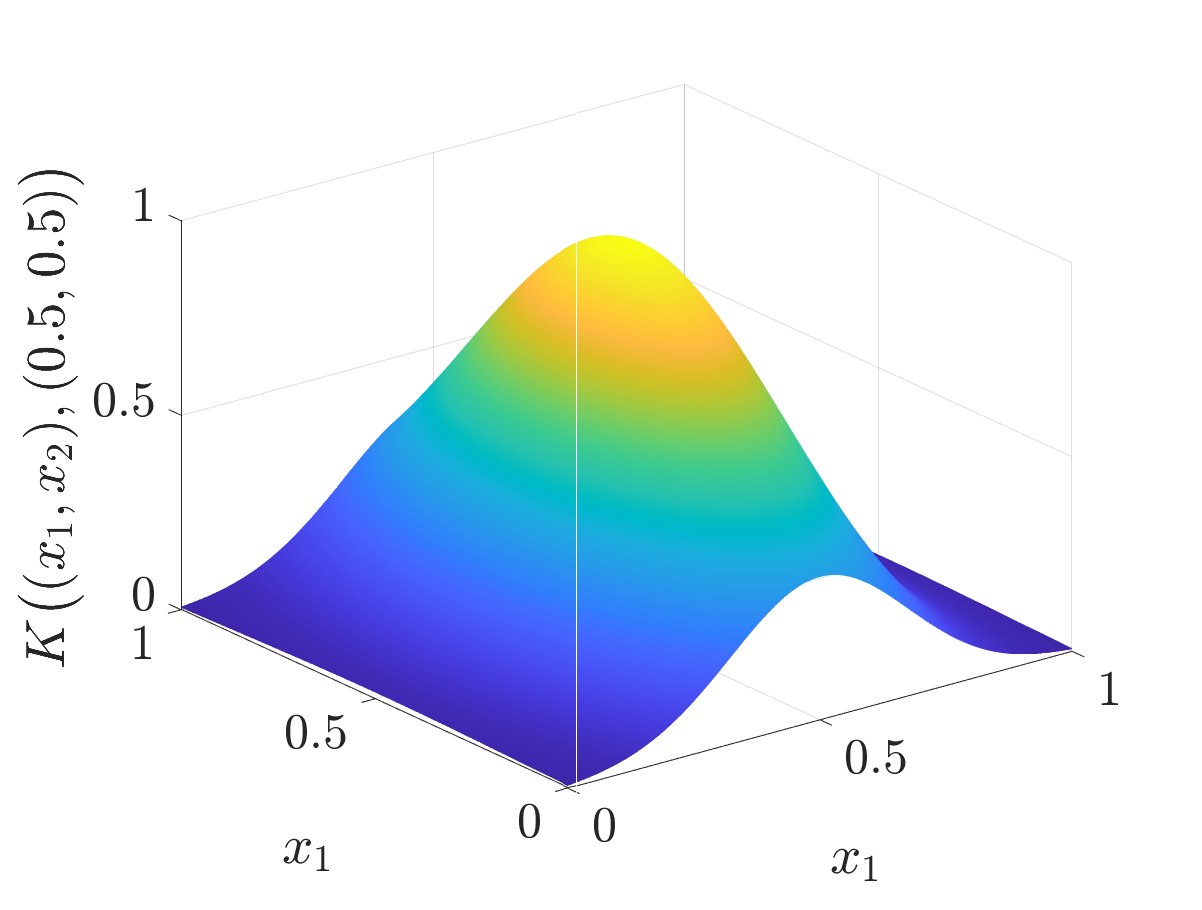
\includegraphics[width=0.38\textwidth]{RK2-sqexpker.eps}
\end{tabular}

\end{frame}

\begin{frame}{Mat\'ern Kernels}
	
\vspace{-5ex}
\begin{tabular}{b{0.5\textwidth}p{0.5\textwidth}}
A popular family of kernels with a range of smoothness depending on $r$ with an associate norm that is not simple to write down:
& 	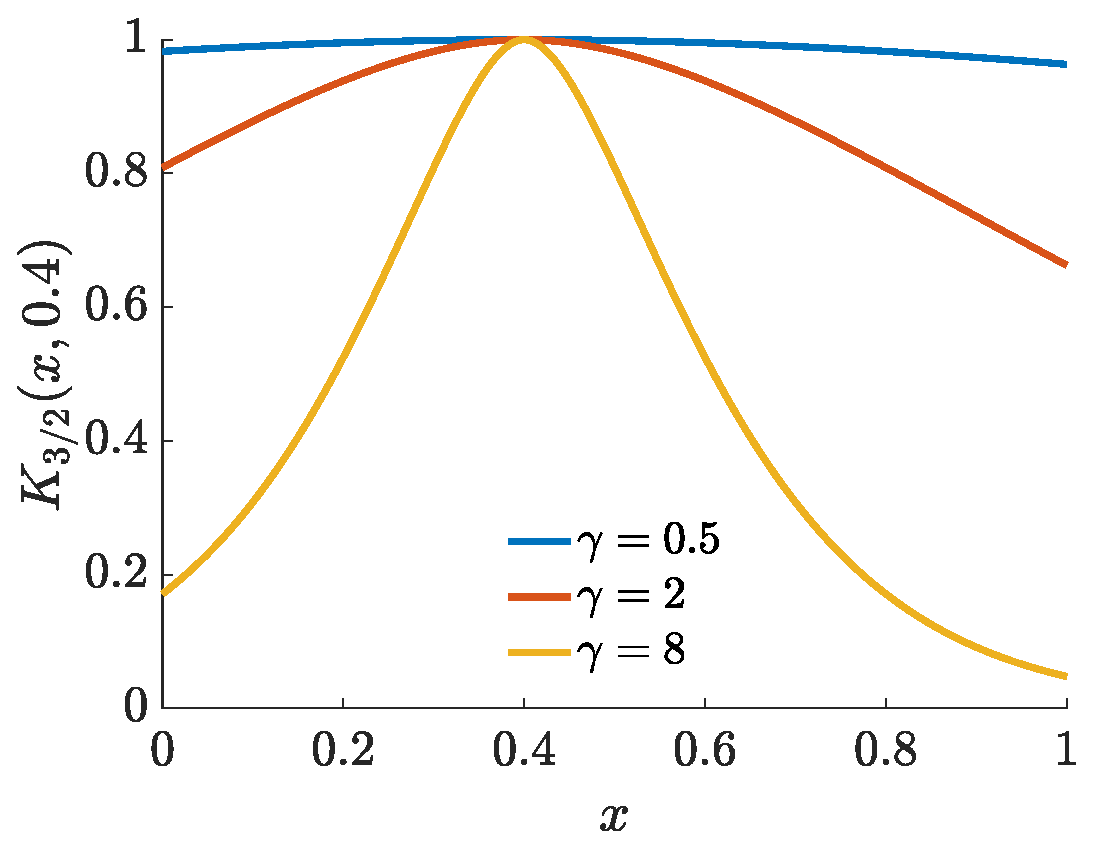
\includegraphics[width=0.45\textwidth]{RK-maternkerthreehalfs.eps}
\end{tabular}
\begin{align*}
	K_r(\vt,\vx) &= A \norm[2]{\vt - \vx}^r \text{Mod Bessel Sec}_r (\gamma \norm[2]{\vt - \vx}) \\
	K_{1/2}(\vt,\vx) & = A_{1/2} \exp(-\gamma\norm[2]{\vt - \vx} )  \quad \alert{\text{not very smooth}} \\
	K_{3/2}(\vt,\vx) & = A_{3/2} (1 + \gamma\norm[2]{\vt - \vx} ) \exp(-\gamma\norm[2]{\vt - \vx} )  \quad \alert{\text{somewhat  smoother}}
\end{align*}


\end{frame}

\begin{frame}{The Centered Discrepancy Kernel \cite{Hic97a}}
	\vspace{-2ex}
	\begin{tabular}{m{0.6\textwidth}m{0.4\textwidth}}
	A reproducing kernel used to analyze cubatures gives the weighted centered discrepancy takes the form
	
	\vspace{-4ex}
	\begin{multline*}
	K(\vt,\vx) : = \prod_{k=1}^d \Bigl[ 1 + \frac {\gamma_k}2 \bigl\{ \abs{t_k - 1/2} + \abs{x_k -1/2} - \abs{t_k-x_k} \bigr\} \Bigr]. \\
	 \vt, \vx \in [0,1]^d
	\end{multline*}

\vspace{-2ex}
which corresponds to the Hilbert space for functions defined on $[0,1]^d$ with the following norm:

	\vspace{-4ex}
		\begin{gather*}
			\norm[2]{D^{\vm} f}^2 := \int_{\reals^d} \abs{\frac{\partial^{\norm[1]{\vm}}f(\vx)}{\partial x_1^{m_1} \cdots \partial x_d^{m_d}}}^2 \bigg \rvert_{x_j = 1/2 \text{ for } m_j = 0} \, \prod_{j \text{ s.t. } m_j > 0} \dif x_j  \\
			\norm{f}^2 : = A \sum_{\norm[\infty]{\vm} \le 1} \frac{\norm[2]{D^{\vm} f}^2}{\gamma_k}
		\end{gather*}
	Mixed partial derivatives of up to order one in each coordinate must be square integrable.
	&
	%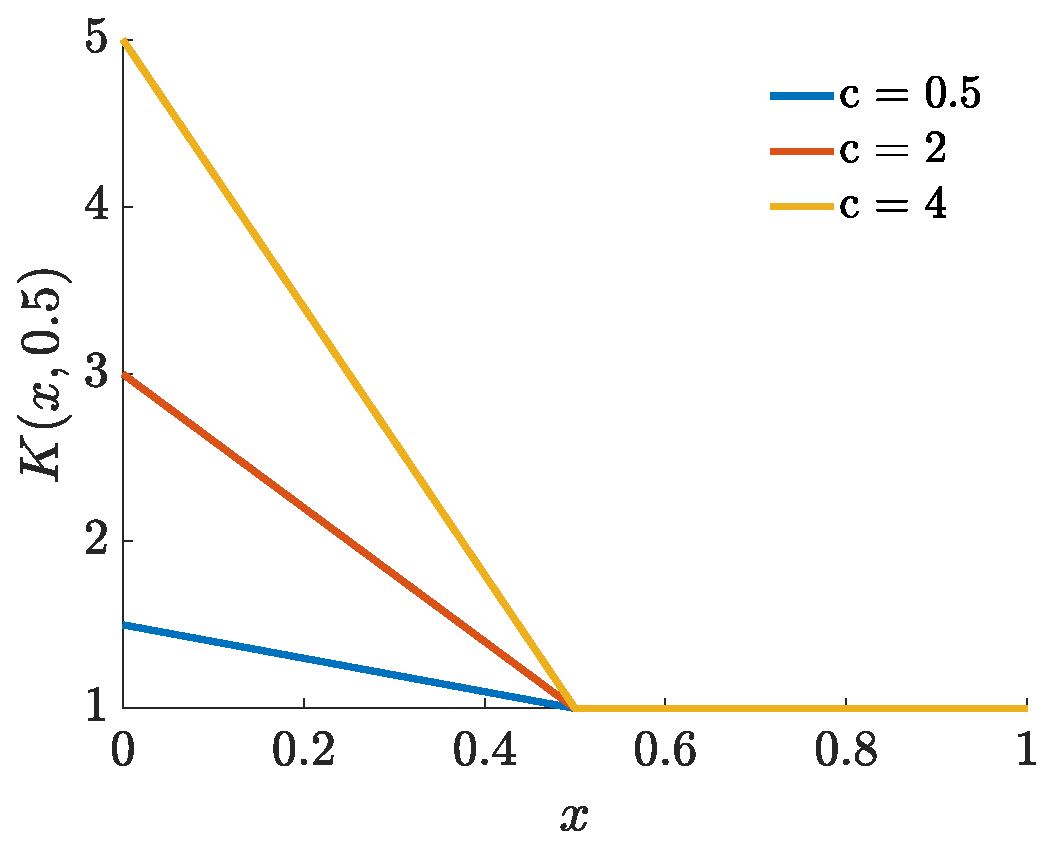
\includegraphics[width=0.38\textwidth]{RK-ctrdiscker.eps}
		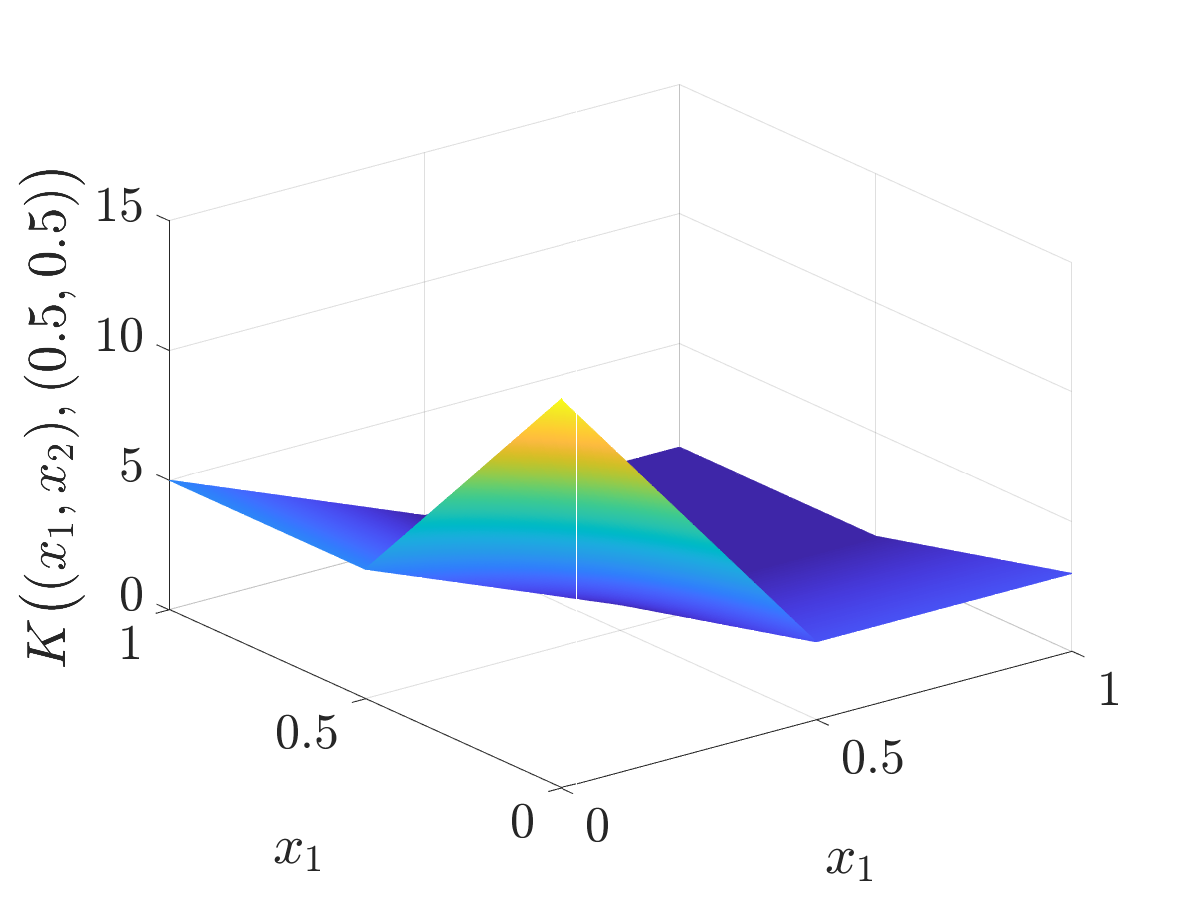
\includegraphics[width=0.38\textwidth]{RK2-ctrdiscker.eps}
		\end{tabular}
\end{frame}


\begin{frame}{The Delta Kernel}
	\vspace{-2ex}
	\begin{tabular}{m{0.5\textwidth}m{0.5\textwidth}}
		A reproducing kernel with an uncountable basis is 
		
		\vspace{-4ex}
		\begin{equation*}
			K(\vt,\vx) : = \begin{cases} 1 + \gamma, & \vt = \vx, \\ 1, & \text{otherwise}, \end{cases}
			\qquad \vt, \vx \in [0,1]^d
		\end{equation*}
		
		\vspace{-2ex}
		which corresponds to the Hilbert space for functions that are a constant everywhere except possibly at a countable number of points.
		
		\vspace{-4ex}
		\begin{gather*}
			I(f) = \int_{[0,1]^d} f(\vx) \, \dif \vx \\
		    \norm{f}^2 : = \abs{I(f)}^2 + \sum_{\vx \in [0,1]^d} \frac{\abs{f(\vx) - I(f)}^2}{\gamma}
		\end{gather*}
	This Hilbert space has an uncountable basis.
		&
		%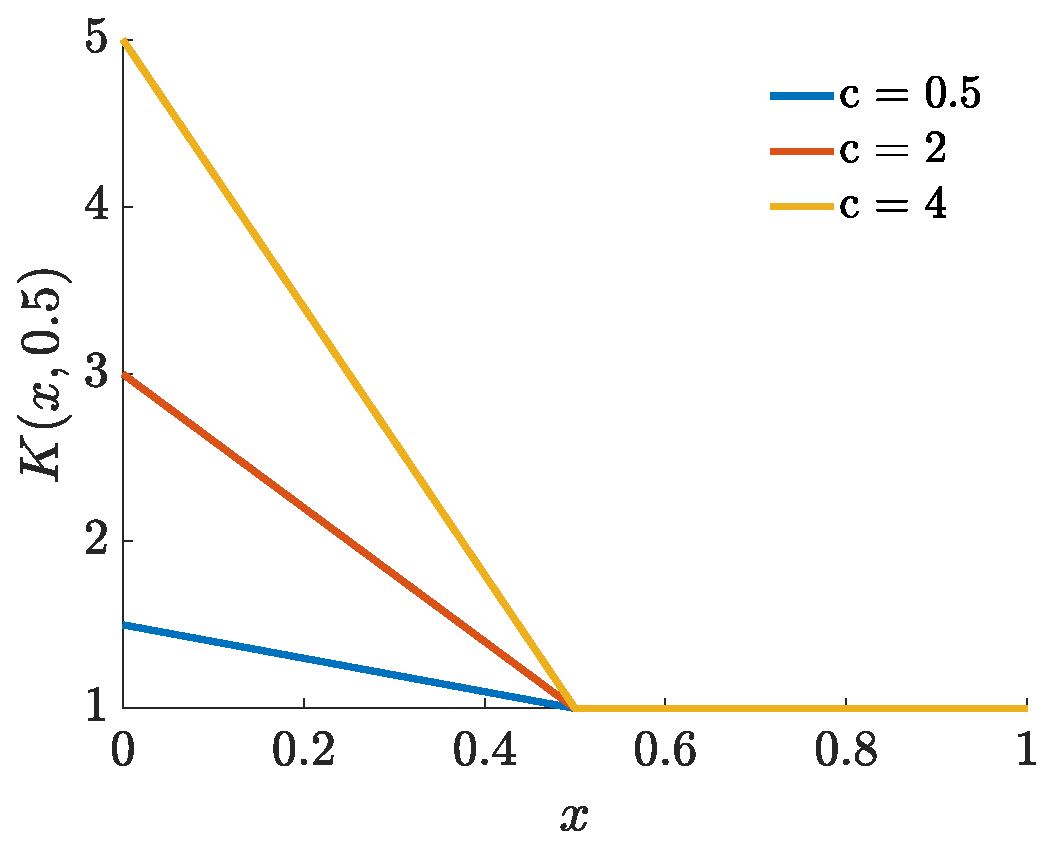
\includegraphics[width=0.38\textwidth]{RK-ctrdiscker.eps}
		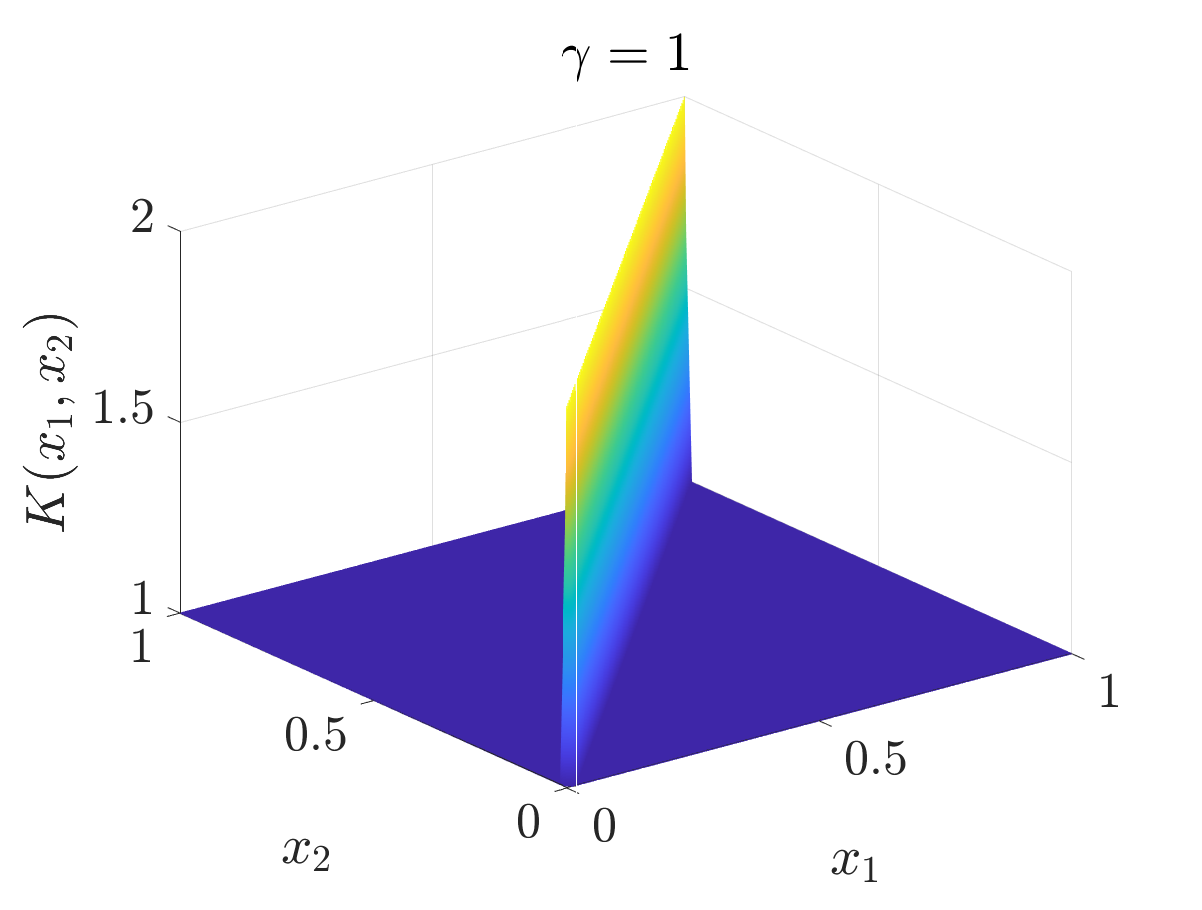
\includegraphics[width=0.38\textwidth]{RK-deltaker.eps}
	\end{tabular}
\end{frame}





%%%%%%%%%%%%%%%%%%%%%%%%%%%%%%%%%%%%%%%%%%
%%%%%%%%%%%%%%%%%%%%%%%%%%%%%%%%%%%%%%%%%%
\section{Assoc Measures}
%%%%%%%%%%%%%%%%%%%%%%%%%%%%%%%%%%%%%%%%%%
%%%%%%%%%%%%%%%%%%%%%%%%%%%%%%%%%%%%%%%%%%




\begin{frame}{Hilbert Spaces of Signed Measures \cite{Hic99a}}
	
	\vspace{-4ex}
	Let $\cm$ be the Hilbert spaced of  measures on $\Omega$ that is the completion of $\{c_1 \delta_{\vx_1} + \cdots + c_n \delta_{\vx_n} :  n \in \naturals, \vc \in \reals^n \}$ under the norm induced by
	\begin{equation*}
		\ip[\cm]{\mu}{\nu} := \int_{\Omega \times \Omega} K(\vt,\vx) \, (\mu \times \nu) (\dif \vt \times \dif \vx)
	\end{equation*}
	and $\delta_{\vx}$ is the Dirac measure, i.e., $\int_{\Omega} f(\vt) \, \delta_\vx(\dif \vt) = f(\vx)$.  There exists a one-to-one and onto, isometric  (I think) mapping $T : \cm \to \cf$ defined as 
		\begin{equation*}
			T(\mu)(\vx) := \int_\Omega K(\vt, \vx) \, \mu(\dif t) \qquad \forall x \in \Omega, \mu \in \cm
		\end{equation*}
such that $\ip{T(\nu)}{f} = \int_\Omega f(\vx) \, \nu (\dif\vx)$.  

If $T(\nu_\vx)$ is the representer for the solution of a differential equation at $\vx$, is $\nu_\vx$ the Green's function?

\end{frame}

\begin{frame}{Can We Findlike the $\mW$ for functions on $\{1, \ldots, d\}$}
	
	\vspace{-4ex}
	Let $\cm$ be the Hilbert spaced of  measures on $\Omega$ that is the completion of $\{c_1 \delta_{\vx_1} + \cdots + c_n \delta_{\vx_n} :  n \in \naturals, \vc \in \reals^n \}$ under the norm induced by
	\begin{equation*}
		\ip[\cm]{\mu}{\nu} := \int_{\Omega \times \Omega} K(\vt,\vx) \, (\mu \times \nu) (\dif \vt \times \dif \vx)
	\end{equation*}
	and $\delta_{\vx}$ is the Dirac measure, i.e., $\int_{\Omega} f(\vt) \, \delta_\vx(\dif \vt) = f(\vx)$.  
	
	Is there a measure $\omega $ on $\Omega \times \Omega$ such that 
	\begin{equation*}
		\int_{\Omega \times \Omega} K(\vt, \vs)K(\vu,\vx) \, \omega(\dif \vs \times \dif \vu)  = K(\vt,\vx) \qquad \forall \vt, \vx \in \Omega?
	\end{equation*}
	This would be like the $\mW$ for functions on $\{1, \ldots, d\}$
	
\end{frame}

\begin{frame}{Separable Hilbert Spaces, i.e., Those with Countable Bases}
	
\vspace{-4ex}
Hilbert spaces of functions on $\Omega$ with countable bases can be written in terms of an $L^2(\Omega)$ basis

\vspace{-4ex}
\[
f(\vx) = \sum_{\vk} \hf(\vk) \varphi_\vk(\vx), \qquad \int_\Omega \varphi_\vk(\vx) \varphi_\vl(\vx)  \, \dif \vx = \delta_{\vk,\vl}
\]

\vspace{-4ex}
and the reproducing kernel is
\vspace{-2ex}
\begin{gather*}
K(\vt,\vx) =  \sum_{\vk} \lambda_\vk \varphi_\vk(\vt) \varphi_\vk(\vx),  \qquad
\text{note that }  \int_\Omega K(\vx,\vx) \, \dif \vx = \sum_{\vk} \lambda_\vk  < \infty, \quad \text{so } \lambda_{\vk} \to 0 \\
\ip{f}{g} := \sum_{\vk} \frac{\hf(\vk) \hg(\vk)}{\lambda_\vk}, \qquad \text{since this implies } 
\ip{K(\cdot,\vx)}{f} := \sum_{\vk} \frac{\lambda_\vk \varphi_\vk(\vx) \hf(k)}{\lambda_\vk} = \sum_{\vk} \varphi_\vk(\vx) \hf(k) =  f(\vx)
\end{gather*}

\vspace{-4ex}
If we formally define the distribution $m(\vx) = \sum_{\vk} \frac{\hf(\vk) \varphi_\vk(\vx)}{\lambda_\vk }$, then

\vspace{-2ex}
\[
\int_{\Omega} K(\vt,\vx) m(\vt) \, \dif \vt = 
\int_{\Omega}  \sum_{\vk,\vl} \lambda_\vk \varphi_\vk(\vt) \varphi_\vk(\vx) 
\frac{\hf(\vl) \varphi_\vl(\vt)}{\lambda_\vl}  \, \dif \vt = 
\sum_{\vk}  \varphi_\vk(\vx) \hf(\vk) = f(\vx)
\]
This $m(\vx) \dif \vx$ seems to be the $\mu(\dif \vx)$ that gets mapped into $f$ \\
It would seem that $W(\vt,\vx) = \sum_{\vk} \frac{\varphi_\vk(\vt) \varphi_\vk(\vx)}{\lambda_\vk}$, which is not a convergent series


\end{frame}





%%%%%%%%%%%%%%%%%%%%%%%%%%%%%%%%%%%%%%%%%%
%%%%%%%%%%%%%%%%%%%%%%%%%%%%%%%%%%%%%%%%%%
\section{Error Bds}
%%%%%%%%%%%%%%%%%%%%%%%%%%%%%%%%%%%%%%%%%%
%%%%%%%%%%%%%%%%%%%%%%%%%%%%%%%%%%%%%%%%%%


\begin{frame}{Error for Approximating Linear Functionals}

\vspace{-4ex}
Suppose that 

\vspace{-2ex}
\begin{itemize}
    \item Linear $\SOL : \cf \to \reals$ is the desired \alert{solution} (integral, derivative at a point, etc.)
    
    \item $\mX = (\vx_1, \ldots, \vx_n)^T$ is the array of \alert{data sites}
    
    \item $\APP_{\mX,\valpha}(f) = \alpha_{1} f(\vx_1) + \cdots + \alpha_{n} f(\vx_n) = \valpha^T f(\mX)$ is the \alert{approximation}
\end{itemize}

\vspace{-2ex}
Then the approximation error has a tight upper bound of
\begin{align*}
    \abs{\underbrace{\SOL(f) - \APP_{\mX,\valpha}(f)}_{\text{linear, bounded}}} &= \abs{\ip{g}{f}} \le \underbrace{\norm{g}}_{\text{badness of $\APP_\mX$}} \, \underbrace{\norm{f}}_{\text{badness of $f$}} \\
    \text{where } g(\vx) &= \bigl(\SOL - \APP_{\mX,\valpha} \bigr) \bigl(K(\cdot,\vx) \bigr) \\
    \norm{g}^2 & = \bigl(\SOL - \APP_{\mX,\valpha} \bigr)^{\cdot\cdot} \Bigl( \bigl(\SOL - \APP_{\mX,\valpha} \bigr)^\cdot\bigl(K(\cdot,\cdot \cdot)\bigr)   \Bigr) \\
    & = \SOL^{\cdot\cdot} \Bigl(\SOL^\cdot\bigl(K(\cdot,\cdot \cdot)\bigr) \Bigr)
    - 2 \valpha^T \SOL\bigl(K(\mX,\cdot) \bigr) + \valpha^T K(\mX,\mX) \valpha
\end{align*}

\vspace{-4ex}
$\APP_\mX$ badness does not require $\ip{\cdot}{\cdot}$, but \alert{only $K$} \hfill
$K(\mX,\cdot) = \bigl(K(\vx_i,\cdot)\bigr)_{i = 1}^n$, $K(\mX,\mX) = \bigl(K(\vx_i,\vx_j)\bigr)_{i,j = 1}^n$ \\
Optimal weights are $\valpha = K(\mX,\mX)^{-1} \SOL\bigl(K(\mX,\cdot) \bigr)$; optimal data sites,  $\mX$, are \alert{hard} nonlinear optimization
\end{frame}

\begin{frame}{An Example of the Cubature Error Bound \cite{Hic97a}}
	
	\vspace{-4ex}
	For the problem and non-optimal approximation
	
	\vspace{-4ex}
	\[
	\SOL(f) = \int_{[0,1]^d} f(\vx) \, \dif \vx, \qquad \APP_{\mX} = \frac 1n \sum_{i=1}^n f(\vx_i),
	\]
	
	\vspace{-3ex}
	and the reproducing kernel
	
	\vspace{-4ex}
	\[
	K(\vt,\vx) : = \prod_{k=1}^d \Bigl[ 1 + \frac {\gamma_k}2 \bigl\{ \abs{t_k - 1/2} + \abs{x_k -1/2} - \abs{t_k-x_k} \bigr\} \Bigr] \qquad \vt, \vx \in [0,1]^d
	\]
	
	\vspace{-3ex}
	 the error bound is $\abs{\SOL(f) -  \APP_{\mX}} \le \BAD(\vx_1, \ldots, \vx_n) \BAD(f)$, where 
	 
	 \vspace{-4ex}
		\begin{multline*}
			\BAD^2(\vx_1, \ldots, \vx_n) = \norm{\text{representer of the error}}^2 \\
			= \left(\frac{13}{12}\right)^d - \frac 2n \sum_{i=1}^n \prod_{k=1}^d \Bigl[ 1 + \frac {\gamma_k}2 \bigl\{ \abs{x_{ik} - 1/2} - \abs{x_{ik}-1/2}^2 \bigr\} \Bigr] \\
			+ \frac 1{n^2} \sum_{i,j=1}^n\prod_{k=1}^d \Bigl[ 1 + \frac 12 \bigl\{ \abs{x_{ik} - 1/2} + \abs{x_{jk} -1/2} - \abs{x_{ik}-x_{jk}} \bigr\}
		\end{multline*}
	
	\vspace{-4ex}
		Requires $\Order(dn^2)$ operations to compute \\ $\BAD(f) =  \norm{f - f(1/2, \ldots, 1/2)}$, which is impractical to compute
\end{frame}


\begin{frame}{Optimal Function Approximation}
	
	\vspace{-4ex}
	Consider function evaluation at $\vx$, i.e., $\SOL_\vx(f)  = f(\vx)$.  In this case,
	
	\vspace{-3ex}
	\[
	\SOL_\vx^{\cdot\cdot} \Bigl(\SOL_\vx^\cdot\bigl(K(\cdot,\cdot \cdot)\bigr) \Bigr) = K(\vx,\vx), \qquad 
	 \SOL_\vx\bigl(K(\mX,\cdot) = K(\mX,\vx)
	\]
	
	\vspace{-3ex}
	and the optimal algorithm is 
	\vspace{-1ex}
	\begin{align*}
	\APP_{\vx,\mX,\opt}(f) &= K(\vx,\mX) K(\mX,\mX)^{-1} f(\mX)\\
	\abs{f(\vx) - K(\vx,\mX) K(\mX,\mX)^{-1} f(\mX)}^2 &\le  
	\bigl[ K(\vx,\vx) 
	- K(\vx,\mX) K(\mX,\mX)^{-1}  K(\mX,\vx) \bigr] \norm{f}^2 \\
	& \le  
	\underbrace{\bigl[ K(\vx,\vx) 
	- K(\vx,\mX) K(\mX,\mX)^{-1}  K(\mX,\vx) \bigr]}_{\text{only depends on }\mX} 
\bignorm{f - \underbrace{K(\cdot,\mX) K(\mX,\mX)^{-1} f(\mX)}_{\text{best approximation to } f}}^2
	\end{align*}
$\APP_{\cdot,\mX,\opt}(f)$ is in the Hilbert space, and even in the span of $K(\cdot,\vx_1), \ldots, K(\cdot,\vx_n)$, so $ \underbrace{K(\cdot,\mX) K(\mX,\mX)^{-1} f(\mX)}_{\text{best approximation}} \perp \underbrace{f - K(\cdot,\mX) K(\mX,\mX)^{-1} f(\mX)}_{\text{error of approximation}}$

The optimal linear approximation for an arbitrary linear functional is just the linear functional applied to the optimal function approximation

$K(\mX,\mX)$ can be \alert{ill-conditioned} for smooth kernels and lots of data
\end{frame}

\begin{frame}{Cardinal Functions}
	To visualize the effect of an additional data point on the function approximation, we plot $\APP_{\cdot,\mX,\opt}(f) = K(\cdot,\mX) K(\mX,\mX)^{-1} f(\mX)$ for $f(\mX) = \ve_i$ (all data are zero but one)
	
	\begin{center}
		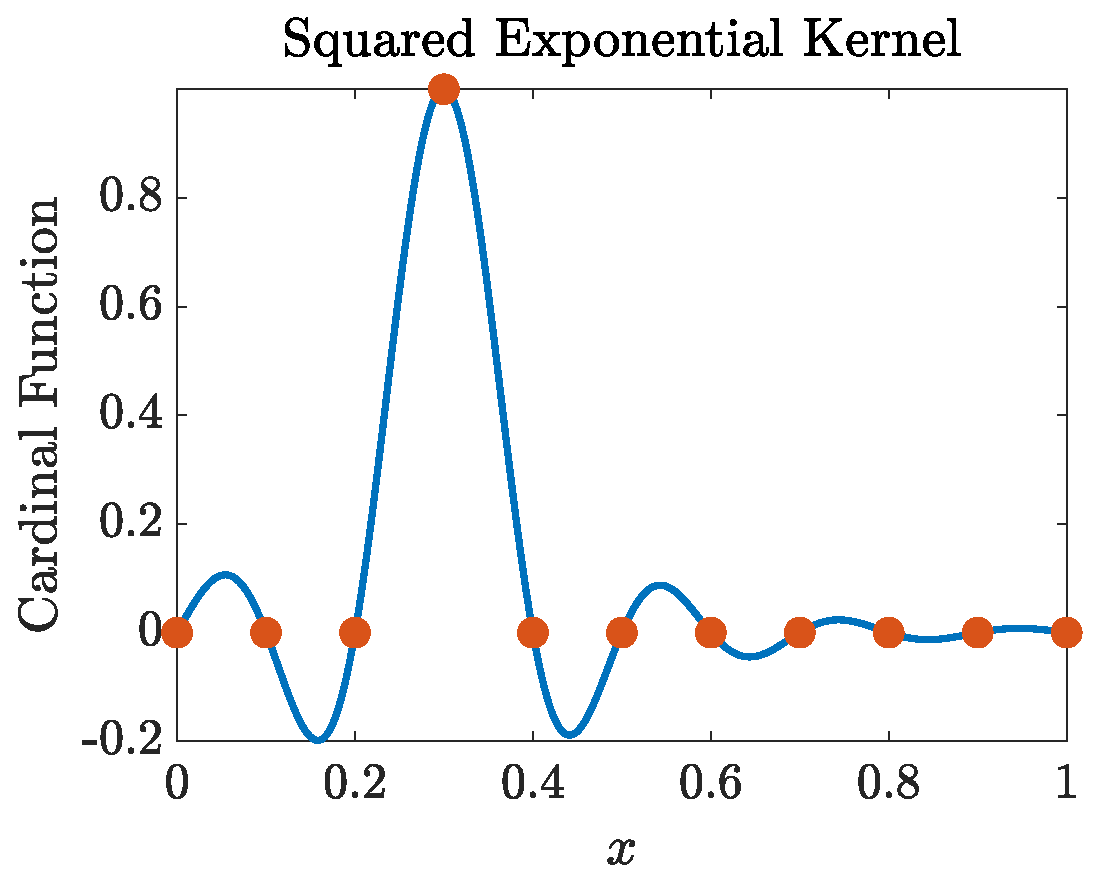
\includegraphics[width = 0.3\textwidth]{Card-sqexpker.eps} \quad
		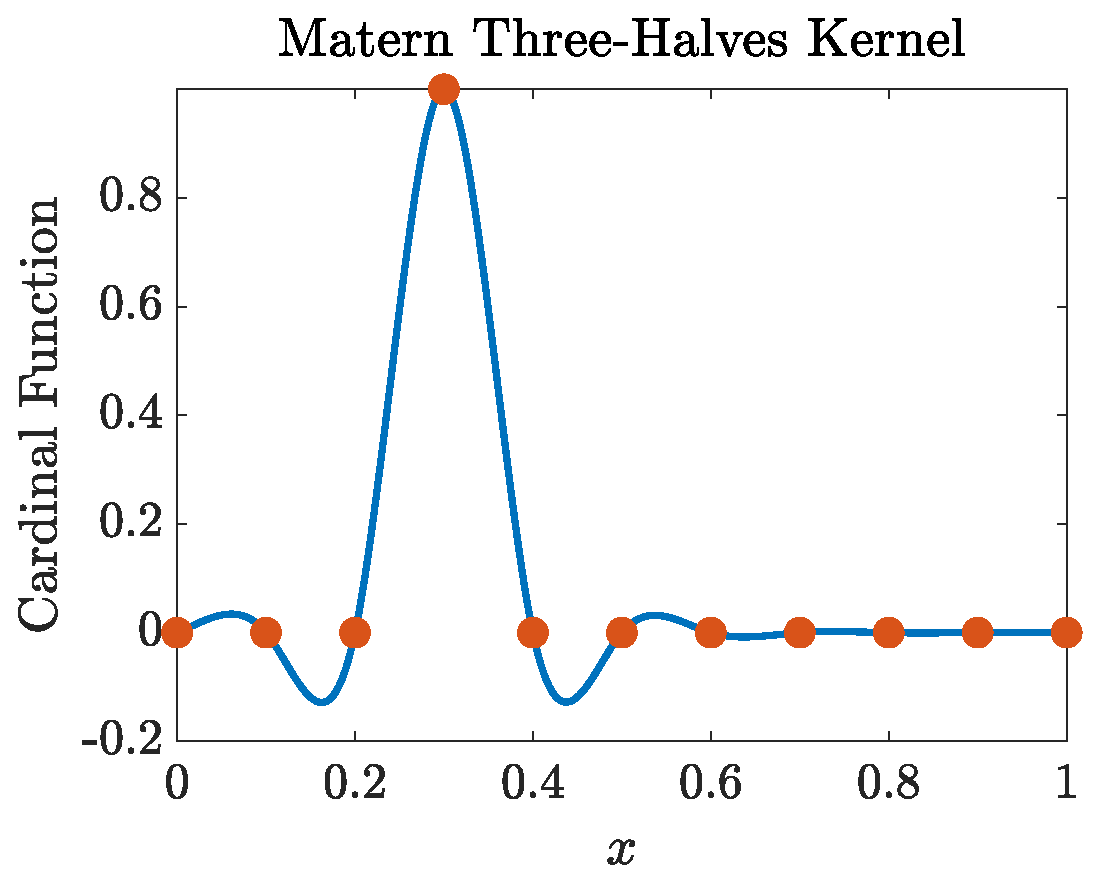
\includegraphics[width = 0.3\textwidth]{Card-maternkerthreehalfs.eps} \quad
		\includegraphics[width = 0.3\textwidth]{Card-ctrdiscker.eps} 
	\end{center}

The cardinal functions of the smoother kernel is more oscillatory
\end{frame}

\begin{frame}{Why Is the Optimal Approximation Linear?}
	\vspace{-4ex}
	Fix $\vx \in \Omega$.  Let 
	\begin{align*}
		\cb_{\mX,f(\mX),R} & = \{ g \in \cf  :  \norm{g}^2 \le R^2 + \norm{ \APP_{\cdot,\mX,\opt}(f)} ^2, \ g(\mX) = f(\mX)\}  \quad \text{functions that look like $f$}\\
		\cb_{\mX,\perp,R} & = \{h \in \cf :  \norm{h} \le R, \ h(\mX) = \vzero\} \qquad \text{functions that vanish at the data sites} \\
		& = \{ h \in \cf :  \norm{h} \le R, \   \ip{h}{K(\cdot,\vx_1)}= \cdots   = \ip{h}{K(\cdot,\vx_n)} = 0 \}
	\end{align*}
Any $g \in \cb_{\mX,f(\mX),R}$ may be written as $g = \APP_{\cdot,\mX,\opt}(f) + g_\perp$ with $g_\perp \in \cb_{\mX,\perp,R}$
	\begin{gather*}
	y_{\opt} := \argmin_{y \in \reals}  \ERR(y) \\
	\ERR(y) : = \max_{g \in \cb_{\mX,f(\mX),R} } \abs{g(\vx) - y} 
	=  \max_{g_\perp \in \cb_{\mX,\perp,R}} \abs{ \APP_{\vx,\mX,\opt}(f) + g_\perp(\vx) - y} 
	\end{gather*}
Since for every $g_\perp \in  \cb_{\mX,\perp,R}$ it also is true that  $-g_\perp \in  \cb_{\mX,\perp,R}$, the optimal choice of $y$ is $\APP_{\vx,\mX,\opt}(f)$.
\end{frame}

\begin{frame}{Tuning the Kernel Parameters}
	Virtually all reproducing kernels have parameters, $\vtheta$, that govern smoothness and shape.  To ensure that your function is typical for the reproducing kernel Hilbert space, $\cf$, one should likely tune these parameters from the function data.  Here is a proposal:
	\[
	 \vtheta_{\opt} = \argmin_{\vtheta} \biggl \{
	\log\bigl(
	\underbrace{f(\mX)^T K_\vtheta(\mX,\mX)^{-1} f(\mX)}_{\text{squared norm of the minimum norm interpolant}}
	\bigr)  
	+  \frac{1}{n} \log(\det(K_\vtheta(\mX,\mX)))
	\biggr \}
	\]
	This corresponds to choosing $\vtheta$ to \alert{minimize} the volume of the ellipsoidal solid in $\reals^n$ consisting of all possible function data whose minimum-norm interpolants have an $\cf_{\vtheta}$-norm no greater than that of the observed interpolant.
	
	It also corresponds to using empirical Bayes when working in the Gaussian process setting with covariance kernels, $K_\vtheta$
	
\end{frame}


\finalthanksnote{These slides are  available at \\  \href{https://speakerdeck.com/fjhickernell/reproducing-kernel-tutorial}{\nolinkurl{speakerdeck.com/fjhickernell/reproducing-kernel-tutorial}}}

\thankyouframe

\begin{frame}{References}
    \printbibliography
\end{frame}



\end{document}





